\usetikzlibrary{arrows.meta}

\chapter{Recursive Types}

%%%%%%%%%%%%%%%%%%%%%%%%%%%%%%%%%%%%%%%%%%%%%%%%%%%%%%%%%%%%%%%%%%%%%%%%%%%%%%%
\section{Iso-recursive Types}

\newcommand\Fold[1]{\texttt{fold}\;#1}
\newcommand\Unfold[1]{\texttt{unfold}\;#1}

\newcommand\Foldv[1]{\texttt{fold}^\textsc{v}\;#1}

Let's take a look at a common data type used in functional programming,
namely lists. They consist of two constructs---nil and cons.
Following those constructs we can try writing a type of lists containing
elements of type $\tau$:

\[
  \texttt{List}\; \tau = \texttt{unit} + (\tau \times \texttt{List}\; \tau)
\]

Writing this type out makes our problem evident---type $\texttt{List}\; \tau$
is present on the right side of this equation.
To solve this problem we need to extend our type system by adding
\emph{recursive types}. We do this by adding a sort of fix construct in
which a variable $\alpha$ is a type of the whole expression and can be used
inside $\tau$.

\[
  \tau \Coloneqq \cdots\mid \mu\alpha\ldotp\tau
\]

According to this definition, we can write our original type of lists as:

\[
  \texttt{List}\; \tau =\mu\alpha\ldotp\texttt{unit} + (\tau \times \alpha)
\]

We should consider a relation between those two types:

\begin{mathpar}
  \mu\alpha\ldotp\tau\and
  \Subst \tau {\mu\alpha\ldotp\tau} \alpha
\end{mathpar}

Thinking of them semantically they should be equal,
but syntactically they are different.
In this chapter we treat them as isomorphic and define two operations that
convert one to the other.

\begin{figure}[H]
    \centering
    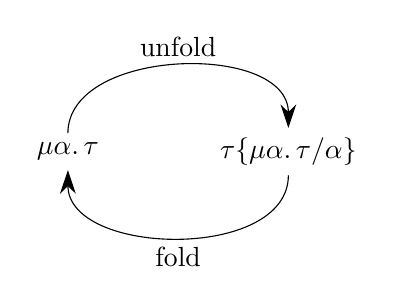
\begin{tikzpicture}[auto, scale=0.7]
        \node (1) at (-2, 0) {$\mu \alpha \ldotp \tau$};
        \node (2) at (2, 0) {$\tau \{\mu \alpha \ldotp \tau / \alpha\}$};

        \draw [->, -{Stealth[length=3mm, width=2mm]}] (1) to [out=90, in=90] node {unfold} (2);
        \draw [->, -{Stealth[length=3mm, width=2mm]}] (2) to [out=270, in=270] node {fold} (1);
    \end{tikzpicture}
    \caption{"Isomorphism" between iso-recursive types}
\end{figure}

With this addition we need to extend a grammar of expressions and values.

\begin{alignat*}{2}
  e & \Coloneqq \cdots\mid\Fold e \mid \Unfold e\\
  v & \Coloneqq \cdots\mid\Foldv v
\end{alignat*}

Together with some reduction and typing rules.

\begin{alignat*}{2}
  \Fold v             & \longrightarrow \Foldv v \\
  \Unfold{(\Foldv v)} & \longrightarrow v
\end{alignat*}


\begin{mathpar}
  \inferrule{\Gamma \vdash e \colon \Subst \tau {\mu\alpha\ldotp\tau} \alpha}
            {\Gamma\vdash \Fold e \colon \mu\alpha\ldotp\tau}

  \inferrule{\Gamma\vdash e \colon \mu\alpha\ldotp\tau}
            {\Gamma \vdash \Unfold e \colon
              \Subst \tau {\mu\alpha\ldotp\tau} \alpha}
\end{mathpar}

We should note that we added a $\Fold e$ as a value instead of $\Unfold e$,
because the former gives a $\mu\alpha\ldotp\tau$
which can't really evaluate further, but the latter can.


%%%%%%%%%%%%%%%%%%%%%%%%%%%%%%%%%%%%%%%%%%%%%%%%%%%%%%%%%%%%%%%%%%%%%%%%%%%%%%%
\section{Local Type Declarations}

\newcommand\FoldDec[2]{\texttt{fold}_#1\;#2}
\newcommand\UnfoldDec[2]{\texttt{unfold}_#1\;#2}
\newcommand\TypeDec[2]{\texttt{type}\;#1\;\texttt{in}\;#2}

\begin{alignat*}{2}
  \tau   & \Coloneqq \alpha\mid\tau\to\tau\mid\cdots \\
  e      & \Coloneqq \cdots\mid\TypeDec\alpha e
             \mid\FoldDec\alpha e \mid\UnfoldDec \alpha e \\
  \Delta & \Coloneqq \cdot\mid\Delta, \alpha \mid \Delta, \alpha = \tau
\end{alignat*}


\begin{mathpar}
  \inferrule{\Delta, \alpha = \tau'; \Gamma \vdash e \colon \tau \\\
             \alpha \not\in \FVars\tau}
             {\Delta; \Gamma \vdash \TypeDec\alpha e \colon \tau}

  \inferrule{\Delta; \Gamma \vdash e \colon \tau \\\
             (\alpha =\tau)\in \Delta}
             {\Delta; \Gamma \vdash \FoldDec\alpha e \colon \alpha}

  \inferrule{\Delta; \Gamma \vdash e \colon \alpha \\\
             (\alpha =\tau)\in \Delta}
             {\Delta; \Gamma \vdash \UnfoldDec\alpha e \colon \tau}
\end{mathpar}

%%%%%%%%%%%%%%%%%%%%%%%%%%%%%%%%%%%%%%%%%%%%%%%%%%%%%%%%%%%%%%%%%%%%%%%%%%%%%%%
\section{Type Reconstruction}

%%%%%%%%%%%%%%%%%%%%%%%%%%%%%%%%%%%%%%%%%%%%%%%%%%%%%%%%%%%%%%%%%%%%%%%%%%%%%%%
\section{Equi-recursive Types}

\newcommand\UnfoldRel{\leadsto}

An another approach to recursive types is called equi-recursive types.
In this approach we treat types $\mu\alpha\ldotp\tau$
and $\Subst \tau {\mu\alpha\ldotp\tau} \alpha$ equal
($\mu\alpha\ldotp\tau \equiv \Subst \tau {\mu\alpha\ldotp\tau} \alpha$)
and we add the following conversion rule to the system.
\begin{mathpar}
  \inferrule{\Gamma \vdash e \;:\; \tau
        \and \tau \equiv \tau'}
            {\Gamma \vdash e \;:\; \tau'}
\end{mathpar}

The type equivalence might be defined as the smallest congruence
containing the rule
\begin{mathpar}
  \inferrule{}
    {\mu\alpha\ldotp\tau \equiv \Subst \tau {\mu\alpha\ldotp\tau} \alpha}
    \textrm{.}
\end{mathpar}
Although such defined type system is sound,
the equivalence relation is too fine-grained making it impractical
and hard to implement.
Consider the type
$\tau = \mu\alpha\ldotp \textsf{Int}\to\textsf{Int}\to\alpha$.
It is a type of functions, that accepts any number of integer values
and greedily ask for more.
From practical point of view,
type $\tau$ should be equivalent to $\textsf{Int} \to \tau$,
but they cannot be equated using inductively defined congruence:
each unfolding of recursive types in $\tau$ gives even number of arrows,
while the number of arrows in $\textsf{Int} \to \tau$ always remain odd.

We define type equivalence as the most coarse-grained relation
that do not relate types that can be differentiated by finite amount of time.
To be more precise, we define it using the notion of \emph{bisimulation}.
Similarly to process calculi and labelled transitions systems we start
with identifying \emph{silent transitions}, which in our case will
be unfolding of a recursive type on a head position.
\begin{mathpar}
  \inferrule{}
    {\mu\alpha\ldotp\tau \UnfoldRel
      \Subst \tau {\mu\alpha\ldotp\tau} \alpha}
\end{mathpar}
If we treat taking of some type component (\emph{e.g.}, left-hand-side
of an arrow) as some non-silent transitions,
we can define a bisimilarity of types.
The specialized definition would be the following.

\begin{defin}
  A binary relation $\mathcal{R}$ on types is called $\emph{simulation}$
  if for each $\tau_1\mathrel{\mathcal{R}} \tau_2$ we have the following:
  \begin{thmenumerate}
  \item if $\tau_1 \UnfoldRel \tau_1'$ then
    $\tau_2 \UnfoldRel^* \tau_2'$
    for some $\tau_2'$
    such that $\tau_1' \mathrel{\mathcal{R}} \tau_2'$;
  \item if $\tau_1$ is of the form $\tau_1' \to \tau_1''$
    then $\tau_2 \UnfoldRel^* \tau_2' \to \tau_2''$
    for some $\tau_2'$ and $\tau_2''$
    such that $\tau_1' \mathrel{\mathcal{R}} \tau_2'$
    and $\tau_1'' \mathrel{\mathcal{R}} \tau_2''$;
  \item \ldots (analogous clauses for other type constructs).
  \end{thmenumerate}
  A relation $\mathcal{R}$ is called \emph{bisimulation}
  if $\mathcal{R}$ and $\mathcal{R}^{-1}$ are simulations.
  A \emph{bisimilarity} (denoted as $\equiv$ or $\simeq$)
  is the largest bisimiulation.
\end{defin}

%%%%%%%%%%%%%%%%%%%%%%%%%%%%%%%%%%%%%%%%%%%%%%%%%%%%%%%%%%%%%%%%%%%%%%%%%%%%%%%
\section{Further Reading}
